
\begin{figure}\center
 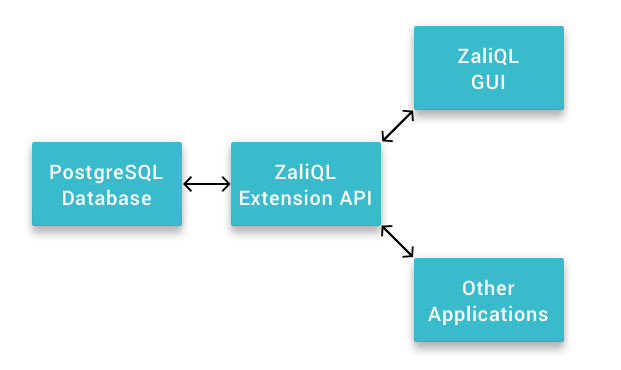
\includegraphics[scale=0.20]{Figures/System-Overview.png}
  \vspace{-3.3mm} \caption{ZaliQL architecture}

  \label{fig:arch}
  \vspace{-3mm}
\end{figure}


\begin{figure} \center
  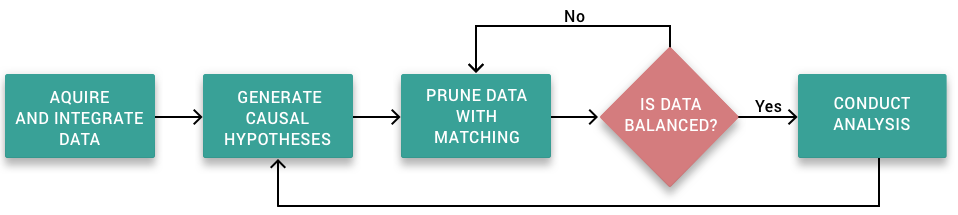
\includegraphics[scale=0.24]{Figures/Matching-Flowchart.png}
  \vspace{-3mm}\caption{Causal analysis workflow}

\label{fig:flowchart}
\vspace{-0.3cm}
\end{figure}

\vspace{-.3cm}

\section{System Architecture}

The overall architecture of \GSQL\ is shown in Fig. \ref{fig:arch}.
% \dans{corey addressed - start by saying that data is stored in a Postgres system}
The API is a set of functions that support causal inference on data stored in a PostgreSQL DBMS. %\footnote{\url{http://postgresql.org/}}
The API will be packaged as a PostgreSQL extension. %and will be released in
%PostgreSQL Extension Network.\footnote{\url{http://pgxn.org/}}
The \GSQL\ API is modeled after the MatchIt and CEM toolkits
\cite{ho2005,iacus2009cem} and includes methods for drawing causal inference from relational data. For demonstration and exploration purposes, \GSQL\ also includes a web GUI
(see Fig. \ref{sfig:demo-tutorial}). %It can be configured with the user's databases URL after they have installed the \GSQL\ Postgres extension. The  GUI be hosted remotely on a server or locally on \ignore{
%The interface consists of three tabs : Setup, Matching Summary, and Analysis.
%}

\ignore{
\dans{We should add more details here: describe the main functions
  that the API supports; mention that they generate and optimize SQL
  queries.}}
